\documentclass[10pt]{beamer}

\usetheme[progressbar=frametitle]{metropolis}
\usepackage{appendixnumberbeamer}
\usepackage{pgfpages}
\usepackage{booktabs}
\usepackage{xcolor}

\usepackage{pgfplots}

\usepgfplotslibrary{dateplot}

\setbeameroption{show notes on second screen=right}
\setbeamertemplate{note page}{\pagecolor{yellow!5}\insertnote}\usepackage{palatino}
\usepackage{xspace}
\newcommand{\themename}{\textbf{\textsc{metropolis}}\xspace}

\title{Labor Markets and Technological Change: Evidence from Electronic Health Records}

\subtitle{Hanna Glenn}
 \date{\today}

\setbeamertemplate{itemize item}{\scalebox{.6}{$\blacktriangleright$ }}     
\setbeamertemplate{itemize subitem}{\scalebox{.8}{$\centerdot$ }} 

\begin{document}

\maketitle

\setbeamercolor{background canvas}{bg=white}

\begin{frame}{Table of Contents}
  \setbeamertemplate{section in toc}[sections numbered]
  \tableofcontents%[hideallsubsections]
  
  \note[item]{Roadmap of the presentation}
\end{frame}



\section[Motivation]{Motivation}

\begin{frame}[fragile]{What is an EHR?}
\begin{itemize}
    \item Technology purchased and implemented by hospitals
\end{itemize}

\begin{itemize}
    \item Used for:
    \vspace{3mm}
    \begin{itemize}
        \item Electronic patient records
        \vspace{3mm}
        \item More complex (and expensive) EHRs allow for decision making assistance
        \vspace{3mm}
        \item Continuing to evolve over time
    \end{itemize}
\end{itemize}

\note[item]{Get everyone on the same page about how to think about EHRs}
\note[item]{A product in the form of technology that is sold to hospitals (and others, but we focus on hospital setting)}
\note[item]{The most standard element of an EHR is that it converts paper records to electronic records}
\note[item]{New elements of EHRs: interropability, patient interface, decision-making assistance}

\end{frame}

\begin{frame}[fragile]{HIT: Great (Expected) Potential in Healthcare}
\begin{alertblock}{Cost Saving}
\begin{itemize}
    \item Possible cost reduction of hundreds of billions of dollars \\ \scriptsize (Hillestad et al 2005, HA)
\end{itemize}
\end{alertblock}

\begin{alertblock}{Quality Improvement}
\begin{itemize}
    \item Improved efficiency, patient safety improvements, physicians have decision support that could prevent unnecessary complications, etc.
    \item Significant policy push for EHR implementation: HITECH Act, 2008 provided financial incentive for hospitals to implement EHRs 
\end{itemize}
\end{alertblock}

\vspace{4mm}

\textcolor{blue}{The percentage of hospitals with basic EHR capability rose from 9$\%$ in 2008 to 84$\%$ in 2015.} \scriptsize (Health IT Dashboard)

\note[item]{Why do we care about EHRs or health information technology in the first place?}

\end{frame}

\begin{frame}[fragile]{What could this mean for physicians?}
Physicians are the ones who put this technology to use, how they respond will partially determine the technology's impacts

\vspace{3mm}


Immediate Effects:
\begin{itemize}
    \item Large startup costs (time, productivity)
    \item Possible loss of autonomy
\end{itemize}

\vspace{4mm}

Long Run Effects:
\begin{itemize}
    \item Productivity could increase
    \item Progressing loss of autonomy as technology progresses
\end{itemize}

\end{frame}

\begin{frame}[noframenumbering]{Physician Response to EHRs}
\begin{center}
    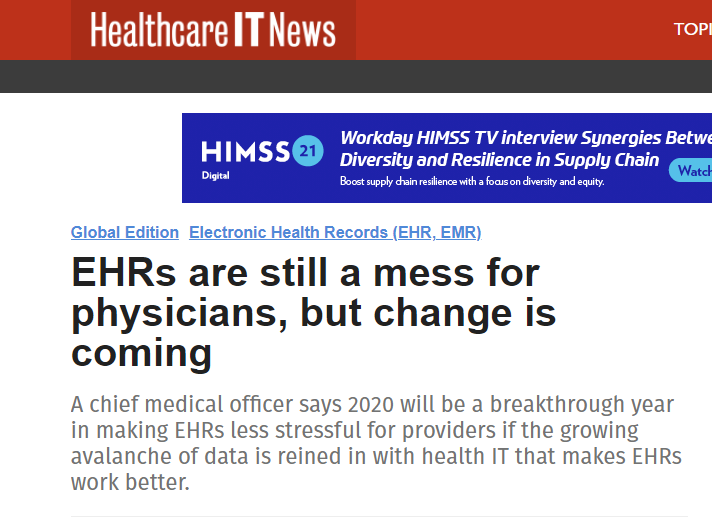
\includegraphics[scale=.4]{graphics/News Clip1.PNG}
\end{center}
\end{frame}

\begin{frame}[noframenumbering]{Physician Response to EHRs}
\begin{center}
    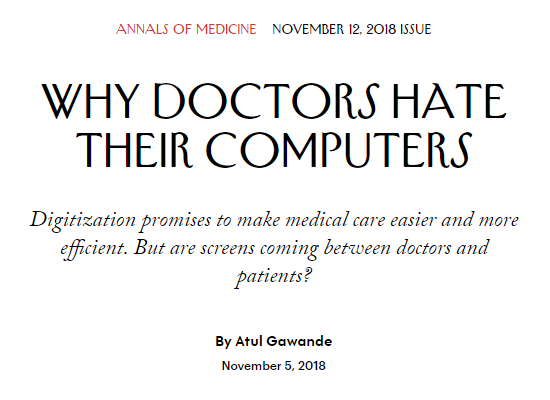
\includegraphics[scale=.5]{graphics/News Clip2.PNG}
\end{center}
\end{frame}

\begin{frame}[noframenumbering]{Physician Response to EHRs}
\begin{center}
    
\includegraphics[scale=.35]{graphics/News Clip3.PNG}
\end{center}
\end{frame}

\begin{frame}{This Paper}

Did EHR implementation in hospitals affect physician labor outcomes?
\begin{itemize}
    \item Intensive Margin / Productivity
    \item Extensive Margin
    \item Hospital $\rightarrow$ Office?
\end{itemize}
\end{frame}


\section{Contribution}

\begin{frame}{Literature}
\footnotesize 
\begin{columns}
    \column{0.34\textwidth}
        \centering
        \underline{ EHR $\rightarrow$ Healthcare }
        \begin{itemize}
            \item Small improvements for severe health conditions \\ \vspace{1mm}
            \tiny(Agha 2014, JHE; McCullough et al 2016, RAND; Meyerhoefer et al, ILRR)
            
            \footnotesize
            
            \item Higher ``levels" of EHR use $\rightarrow$ decline in quality of care\\ \vspace{1mm}
            \tiny (Appari et al 2013)
            
            \footnotesize 
            
            \item No decrease in cost \\ \vspace{1mm}
            \tiny (Agha 2014, JHE; Dranove et al 2019; AEJ) 
            
            \footnotesize
            
            \item Productivity and opinion about EHRs varies drastically \\ \vspace{1mm}
            \tiny (Hitt $\&$ Tambe 2016, Butler $\&$ Johnson 2016, Meyerhoefer et al 2016)
            
        \end{itemize}

    \column{0.33\textwidth}
    \color{gray}
        \centering
        \underline{ Technology $\rightarrow$ Labor }
        \begin{itemize}
        \color{gray}
            \item Erosion effect vs. wage effect \\ \vspace{1mm}
            \tiny (Zeira $\&$ Joseph 2011)
            
            \footnotesize
            
            \item Cause retirement? \\ \vspace{1mm}
            \tiny (Schleife 2006, Cavapozzi et al 2013, Roger et al 2006, Friedburg 2003)
            
            \footnotesize
            
            \item Older, well educated members of labor force exited at higher rates due to computerization \\ \vspace{1mm}
            \tiny (Willis and Hudomiet 2020)
        \end{itemize}
        
        
    \column{0.33\textwidth}
        \color{gray}
        \centering
        Physician Labor \underline{ Determinants }
        \begin{itemize}
        \color{gray}
            \item Physicians not very responsive to wage changes in terms of hours worked \\ \vspace{1mm}
            \tiny (Baltagi et al 2005, Sloan 2018)
            
            \footnotesize
            
            \item Peronal life factors matter more for retirement than work conditions \\ \vspace{1mm}
            \tiny (Bahrami 2002)
            
            \footnotesize
            
            \item Physician burnout: early retirement and less hours worked \\ \vspace{1mm} 
            \tiny (Dewa et al 2014)
        \end{itemize}
        
        
\end{columns}
\end{frame}


\begin{frame}[noframenumbering]{Literature}
\footnotesize 
\begin{columns}
    \column{0.34\textwidth}
    \color{gray}
        \centering
        \underline{ EHR $\rightarrow$ Healthcare }
        \begin{itemize}
        \color{gray}
            \item Small improvements for severe health conditions \\ \vspace{1mm}
            \tiny(Agha 2014, JHE; McCullough et al 2016, RAND; Meyerhoefer et al, ILRR)
            
            \footnotesize
            
            \item Higher ``levels" of EHR use $\rightarrow$ decline in quality of care\\ \vspace{1mm}
            \tiny (Appari et al 2013)
            
            \footnotesize 
            
            \item No decrease in cost \\ \vspace{1mm}
            \tiny (Agha 2014, JHE; Dranove et al 2019; AEJ) 
            
            \footnotesize
            
            \item Productivity and opinion about EHRs varies drastically \\ \vspace{1mm}
            \tiny (Hitt $\&$ Tambe 2016, Butler $\&$ Johnson 2016, Meyerhoefer et al 2016)
            
        \end{itemize}
        
    \column{0.33\textwidth}
        \centering
        \underline{ Technology $\rightarrow$ Labor }
        \begin{itemize}
            \item Erosion effect vs. wage effect \\ \vspace{1mm}
            \tiny (Zeira $\&$ Joseph 2011)
            
            \footnotesize
            
            \item Cause retirement? \\ \vspace{1mm}
            \tiny (Schleife 2006, Cavapozzi et al 2013, Roger et al 2006, Friedburg 2003)
            
            \footnotesize
            
            \item Older, well educated members of labor force exited at higher rates due to computerization \\ \vspace{1mm}
            \tiny (Willis and Hudomiet 2020)
        \end{itemize}
        
        
    \column{0.33\textwidth}
    \color{gray}
        \centering
        Physician Labor \underline{ Determinants }
        \begin{itemize}
        \color{gray}
            \item Physicians not very responsive to wage changes in terms of hours worked \\ \vspace{1mm}
            \tiny (Baltagi et al 2005, Sloan 2018)
            
            \footnotesize
            
            \item Peronal life factors matter more for retirement than work conditions \\ \vspace{1mm}
            \tiny (Bahrami 2002)
            
            \footnotesize
            
            \item Physician burnout: early retirement and less hours worked \\ \vspace{1mm} 
            \tiny (Dewa et al 2014)
        \end{itemize}
\end{columns}
\end{frame}

\begin{frame}[noframenumbering]{Literature}
\footnotesize 
\begin{columns}
    \column{0.34\textwidth}
    \color{gray}
        \centering
        \underline{ EHR $\rightarrow$ Healthcare }
        \begin{itemize}
        \color{gray}
            \item Small improvements for severe health conditions \\ \vspace{1mm}
            \tiny(Agha 2014, JHE; McCullough et al 2016, RAND; Meyerhoefer et al, ILRR)
            
            \footnotesize
            
            \item Higher ``levels" of EHR use $\rightarrow$ decline in quality of care\\ \vspace{1mm}
            \tiny (Appari et al 2013)
            
            \footnotesize 
            
            \item No decrease in cost \\ \vspace{1mm}
            \tiny (Agha 2014, JHE; Dranove et al 2019; AEJ) 
            
            \footnotesize
            
            \item Productivity and opinion about EHRs varies drastically \\ \vspace{1mm}
            \tiny (Hitt $\&$ Tambe 2016, Butler $\&$ Johnson 2016, Meyerhoefer et al 2016)
            
        \end{itemize}
        
    \column{0.33\textwidth}
    \color{gray}
        \centering
        \underline{ Technology $\rightarrow$ Labor }
        \begin{itemize}
        \color{gray}
            \item Erosion effect vs. wage effect \\ \vspace{1mm}
            \tiny (Zeira $\&$ Joseph 2011)
            
            \footnotesize
            
            \item Cause retirement? \\ \vspace{1mm}
            \tiny (Schleife 2006, Cavapozzi et al 2013, Roger et al 2006, Friedburg 2003)
            
            \footnotesize
            
            \item Older, well educated members of labor force exited at higher rates due to computerization \\ \vspace{1mm}
            \tiny (Willis and Hudomiet 2020)
        \end{itemize}
        
        
    \column{0.33\textwidth}
        \centering
        Physician Labor \underline{ Determinants }
        \begin{itemize}
            \item Physicians not very responsive to wage changes in terms of hours worked \\ \vspace{1mm}
            \tiny (Baltagi et al 2005, Sloan 2018)
            
            \footnotesize
            
            \item Peronal life factors matter more for retirement than work conditions \\ \vspace{1mm}
            \tiny (Bahrami 2002)
            
            \footnotesize
            
            \item Physician burnout: early retirement and less hours worked \\ \vspace{1mm} 
            \tiny (Dewa et al 2014)
        \end{itemize}
\end{columns}
\end{frame}





\section{Data}


\begin{frame}{What I Want to Capture}
\begin{itemize}
    \item Initial Implementation
    \vspace{3mm}
    \begin{itemize}
        \item Productivity gains/losses?
        \vspace{3mm}
        \item Retirement or change in place of work?
        \vspace{3mm}
    \end{itemize}
    \item Do the effects change over time after the technology is implemented?

\end{itemize}


\end{frame}

\begin{frame}{About the Data}
    Main measurements come from \underline{CMS Shared Patient Data} (2009-2015)
    \begin{itemize}
        \item Lists 2 NPIs and the number of billings those two entities shared
    \end{itemize}
    \vspace{3mm}
    
    How I use it:
    \begin{itemize}
        \item Limit the NPIs to physician-hospital pairs, where physicians are PCPs, internists, hospitalists
        \item Limit the billings to those which occur in the same day
        \item Only keep pairs with sufficient number of billings together to suggest a close relationship between physician and hospital
        \item Aggregate to the physician level to avoid spillover effects
    \end{itemize}
\end{frame}


\begin{frame}{Measures of Physician Labor Market Decisions}


     Hospital patients: 
    \begin{itemize}
        \item Sum of shared patients with all hospitals
    \end{itemize}
     
     \vspace{4mm}
     
     Indicator for switching work setting:
    \begin{itemize}
        \item Positive billings shared with all entities but shared entities with hospitals becomes 0
        \item Database of office-based physicians
    \end{itemize}
    
    \vspace{4mm}
    
    \textcolor{gray}
     {Indicator for retirement/ leaving the labor force}

\end{frame}

\begin{frame}{Measure of EHR Use}

Physician-level treatment variable that captures exposure to \textit{any} EHR
\vspace{3mm}
\begin{itemize}
    \item Individual hospital EHR use comes from AHA survey
    \vspace{3mm}
    \item Treatment turns on the first time any of the shared hospitals implements an EHR
\end{itemize}
\end{frame}


\begin{frame}{Other Characteristics}

Medical school graduation date: \underline{Physician Compare}

\vspace{5mm}

Average size of hospital worked with (measured in beds), average hospital days operating: \underline{AHA Survey}
\end{frame}

\begin{frame}{Summary Statistics}
\centering
    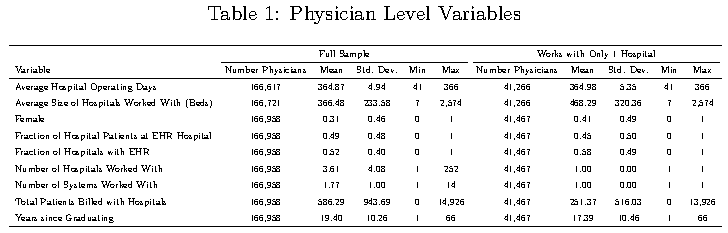
\includegraphics[scale=.8]{Objects/sumstats.pdf}
    
    \note[item]{Need to divide n by 7 to get actual number of physicians}
\end{frame}

\begin{frame}{Physician EHR Use}
    \centering
    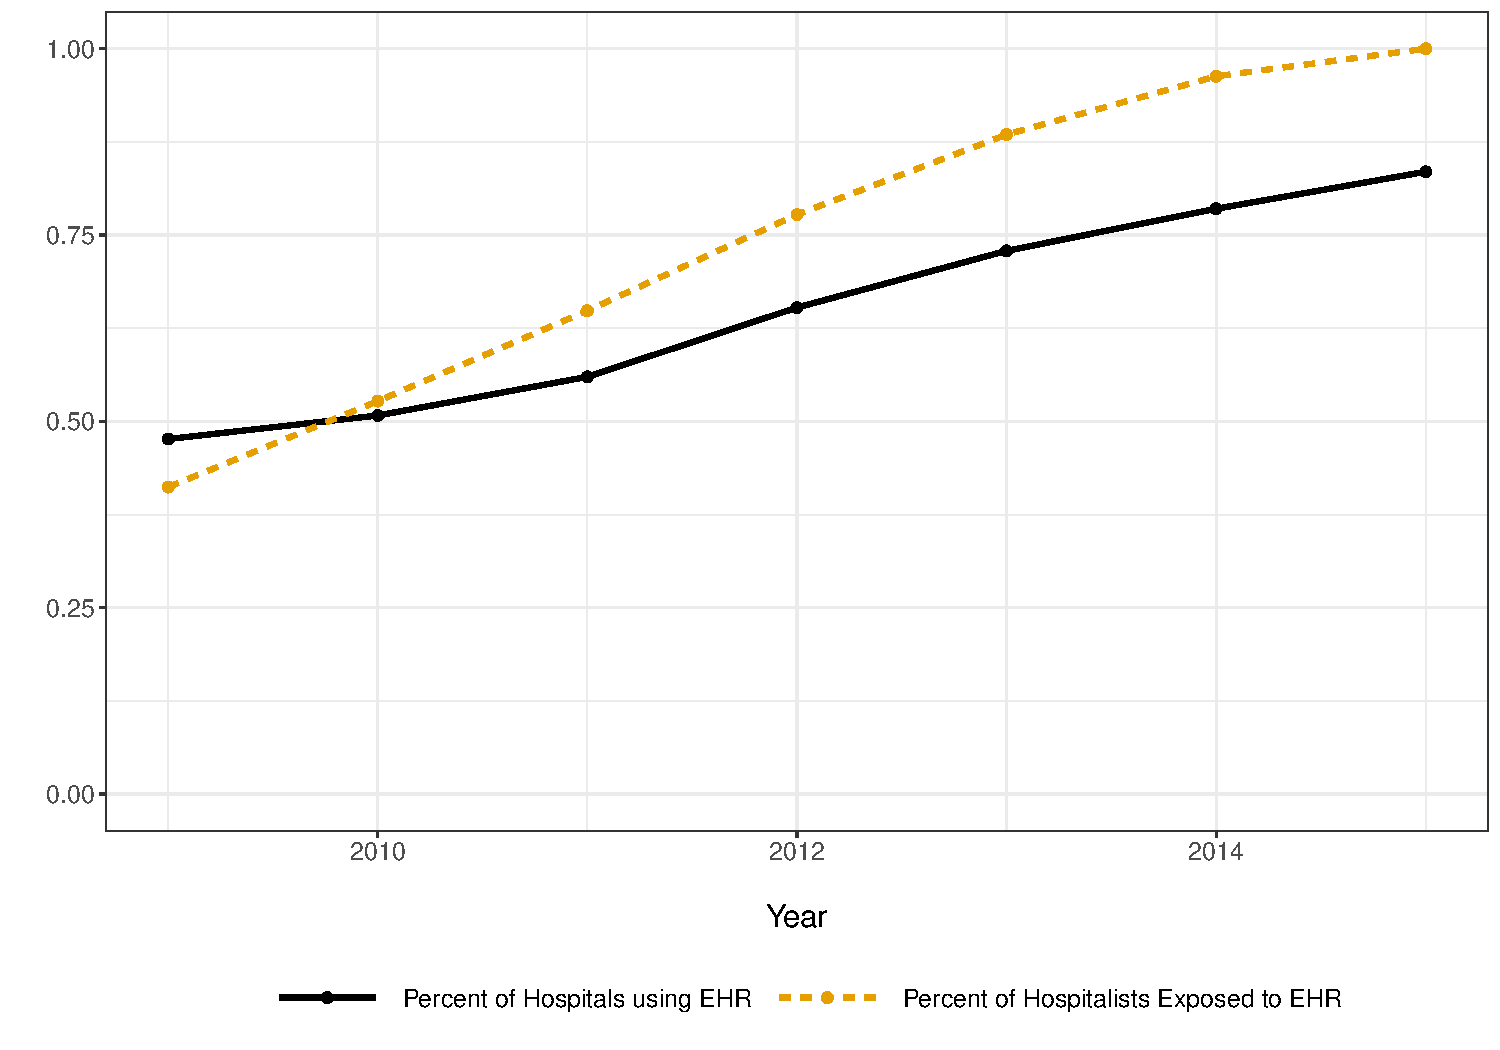
\includegraphics[scale=.5]{Objects/sum_stats_year.pdf}
\end{frame}


\section{Analysis}

\begin{frame}{Event Study}
\begin{equation*}
    y_{it}=\alpha_i+\delta_t+q_{it}'\lambda+\sum_{k=-5}^5 \beta_kz_{i,t-k} + \varepsilon_{it}
\end{equation*}

    
\end{frame}

\section{Results}


\begin{frame}{Dep. Variable: Patients Billed with Hospitals}
\begin{figure}[ht]
        \begin{minipage}[b]{0.47\linewidth}
            \centering
            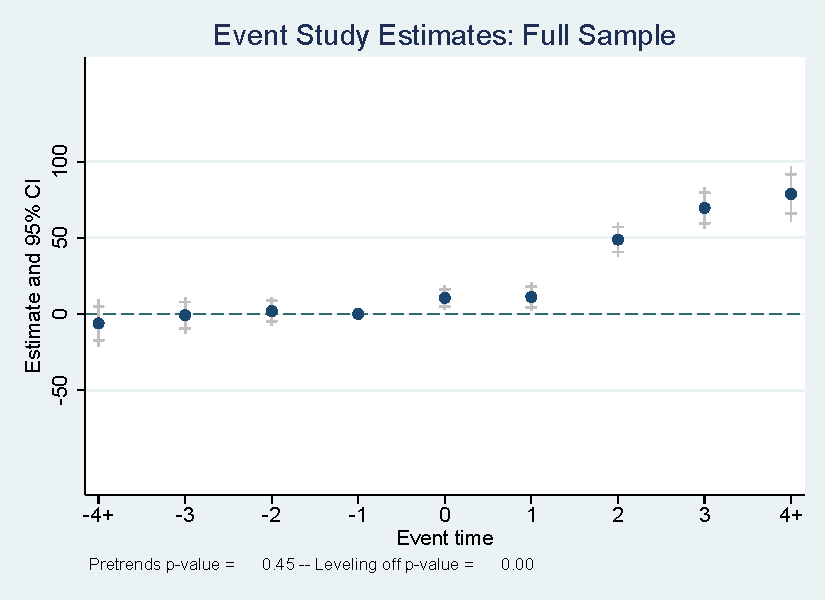
\includegraphics[width=\textwidth]{Objects/xtevent_fullsample.pdf}
            \caption{\small All Physicians\\}
        \end{minipage}
        \hspace{0.2cm}
        \begin{minipage}[b]{0.47\linewidth}
            \centering
            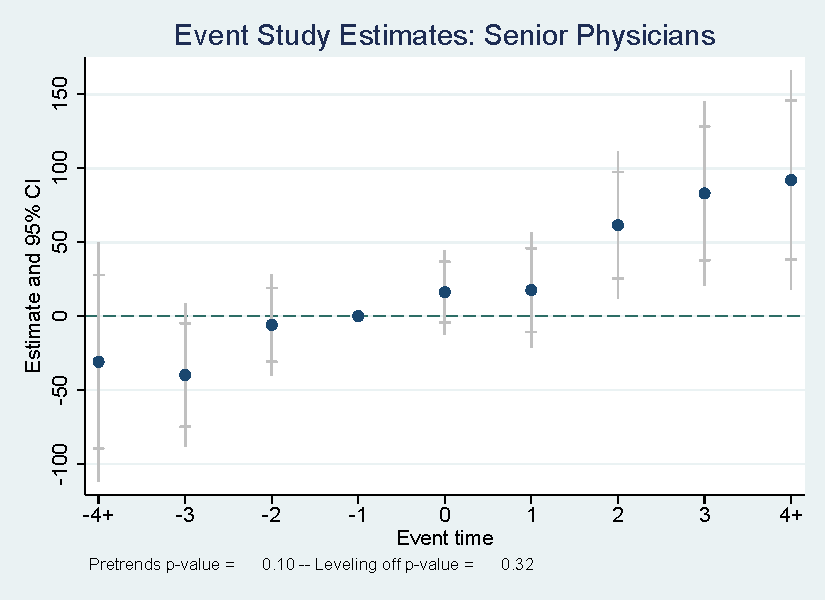
\includegraphics[width=\textwidth]{Objects/xtevent_oldsample.pdf}
            \caption{\small Phys. $>$ 35 yrs Experience}
        \end{minipage}
    \end{figure}
\end{frame}

\begin{frame}{Dep. Variable: Patients Billed with Hospitals}
\begin{figure}[ht]
        \begin{minipage}[b]{0.47\linewidth}
            \centering
            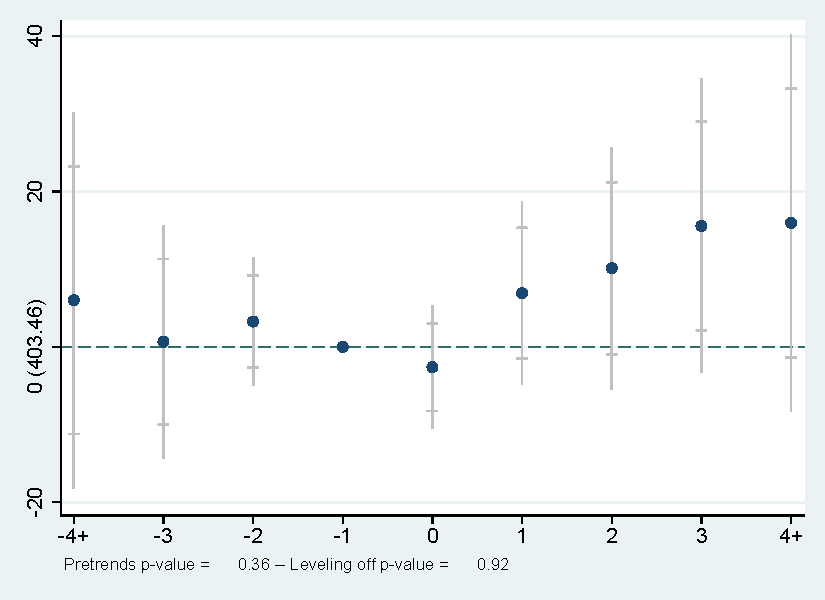
\includegraphics[width=\textwidth]{Objects/xtevent_hosp_fullsample.pdf}
            \caption{\small All Physicians \\(Only 1 Hospital)}
        \end{minipage}
        \hspace{0.2cm}
        \begin{minipage}[b]{0.47\linewidth}
            \centering
            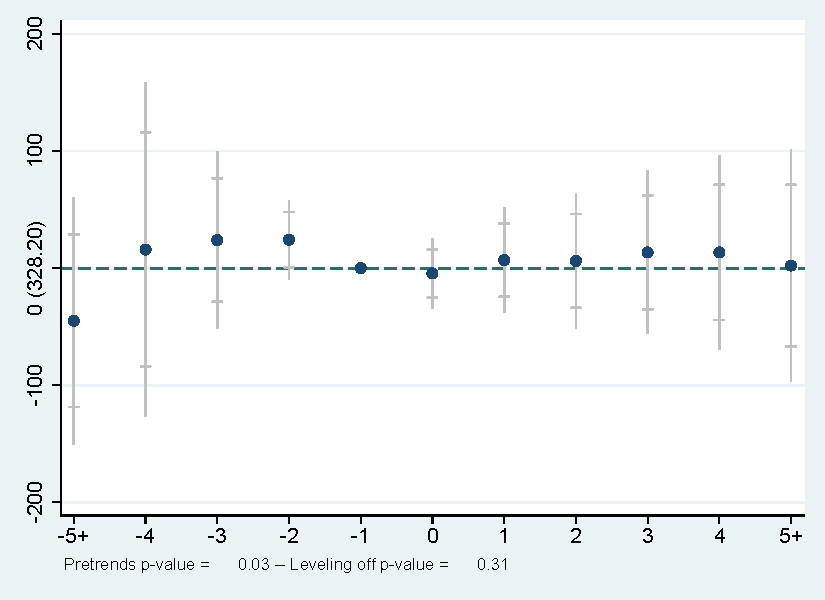
\includegraphics[width=\textwidth]{Objects/xtevent_hosp_oldsample.pdf}
            \caption{\small Phys. $>$ 35yrs\\ (Only 1 Hospital)}
        \end{minipage}
    \end{figure}
\end{frame}


\begin{frame}{Dep. Variable: Probability of Billing, but not With Hospitals}
\begin{figure}[ht]
        \begin{minipage}[b]{0.47\linewidth}
            \centering
            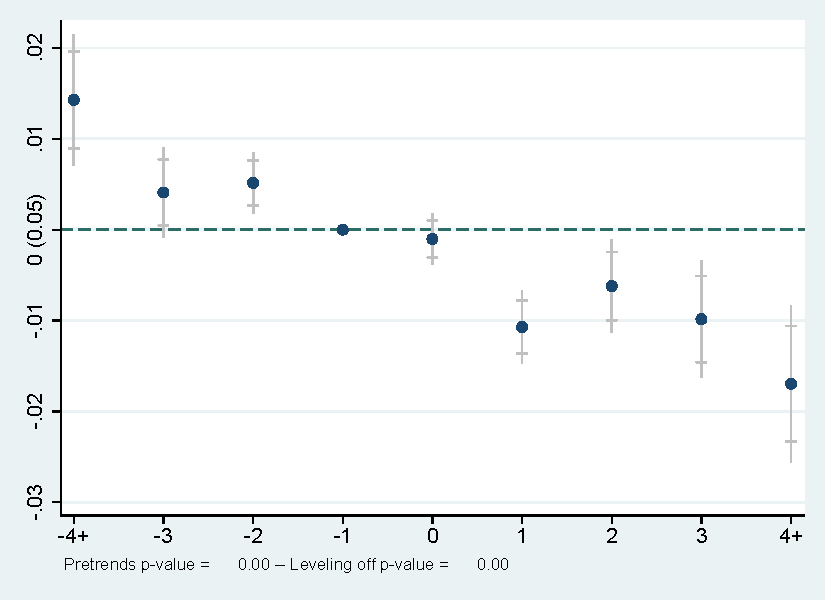
\includegraphics[width=\textwidth]{Objects/xtevent_fullsample_ind.pdf}
            \caption{\small All Physicians}
        \end{minipage}
        \hspace{0.2cm}
        \begin{minipage}[b]{0.47\linewidth}
            \centering
            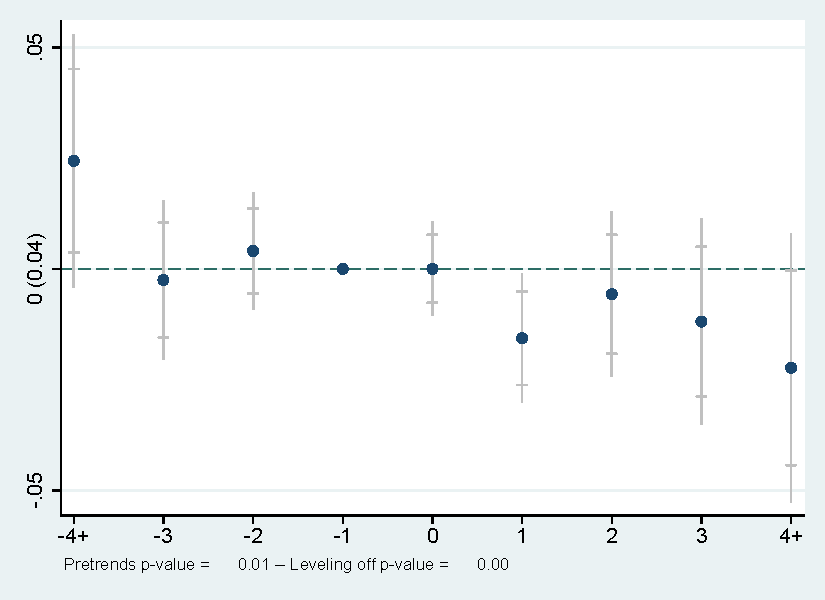
\includegraphics[width=\textwidth]{Objects/xtevent_oldsample_ind.pdf}
            \caption{\small Phys. $>$ 35yrs Experience}
        \end{minipage}
    \end{figure}
\end{frame}


\begin{frame}{Dep. Variable: Probability of Billing, but not With Hospitals}
\begin{figure}[ht]
        \begin{minipage}[b]{0.47\linewidth}
            \centering
            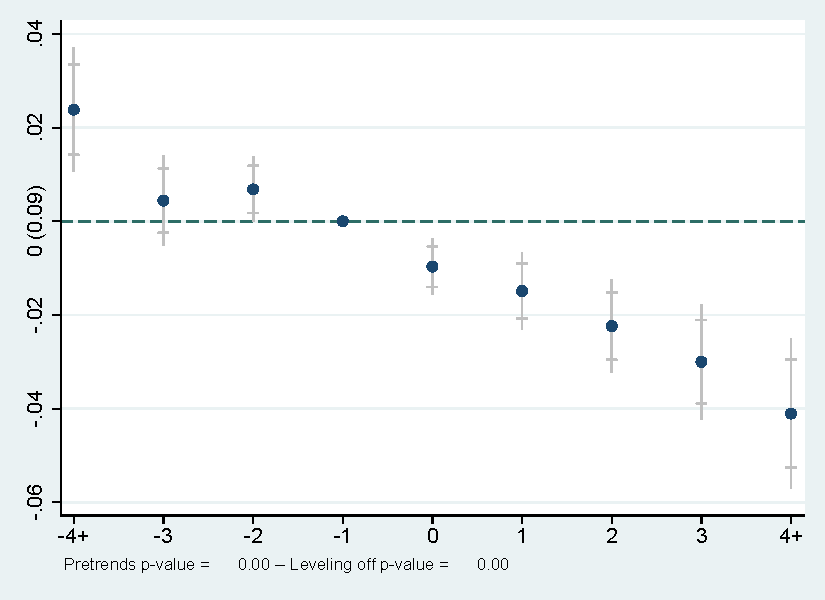
\includegraphics[width=\textwidth]{Objects/xtevent_hosp_fullsample_ind.pdf}
            \caption{\small All Physicians \\(Only 1 Hospital)}
        \end{minipage}
        \hspace{0.2cm}
        \begin{minipage}[b]{0.47\linewidth}
            \centering
            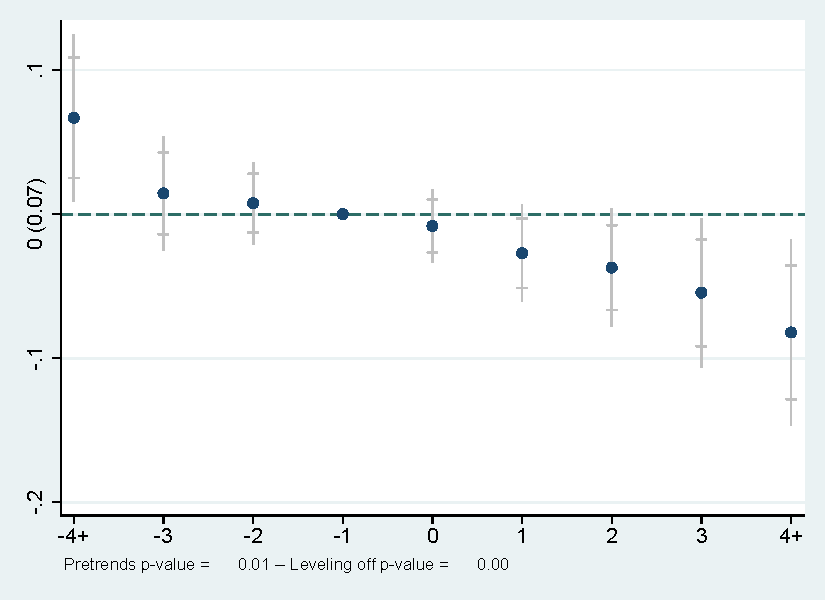
\includegraphics[width=\textwidth]{Objects/xtevent_hosp_oldsample_ind.pdf}
            \caption{\small Phys. $>$ 35yrs Experience\\ (Only 1 Hospital)}
        \end{minipage}
    \end{figure}
\end{frame}

\begin{frame}{Dep. Variable: Appears in Office-Based Data}
\begin{figure}[ht]
        \begin{minipage}[b]{0.47\linewidth}
            \centering
            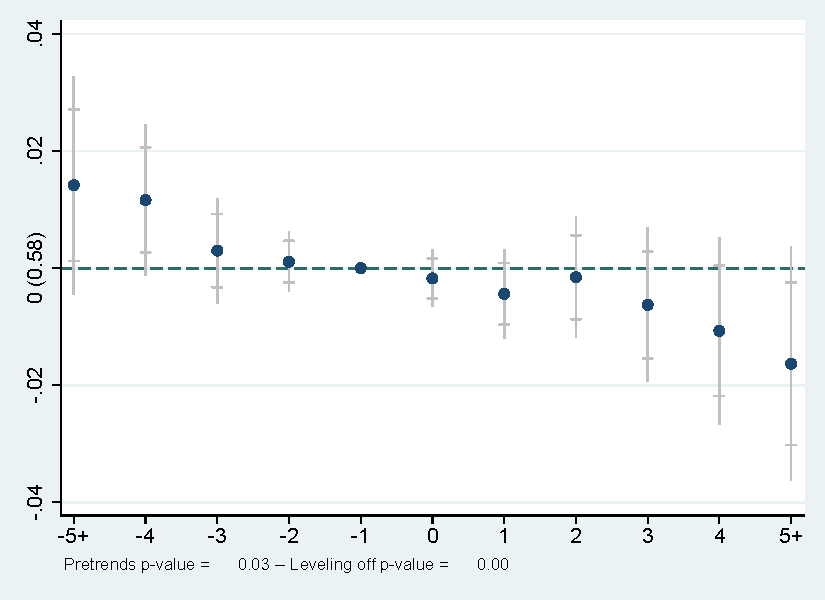
\includegraphics[width=\textwidth]{Objects/xtevent_fullsample_office.pdf}
            \caption{\small All Physicians}
        \end{minipage}
        \hspace{0.2cm}
        \begin{minipage}[b]{0.47\linewidth}
            \centering
            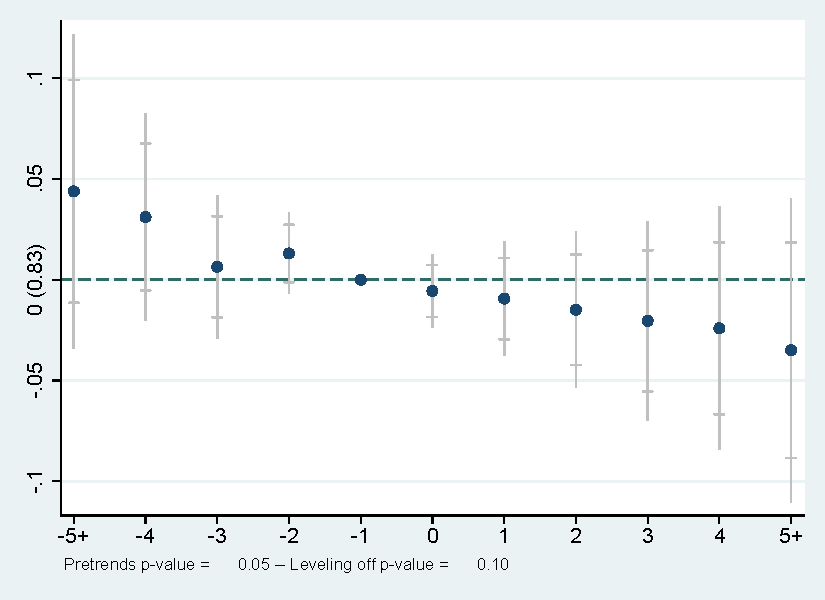
\includegraphics[width=\textwidth]{Objects/xtevent_oldsample_office.pdf}
            \caption{\small Phys.$>$35yrs Experience}
        \end{minipage}
    \end{figure}
\end{frame}


\begin{frame}{Dep. Variable: Appears in Office-Based Data}
\begin{figure}[ht]
        \begin{minipage}[b]{0.47\linewidth}
            \centering
            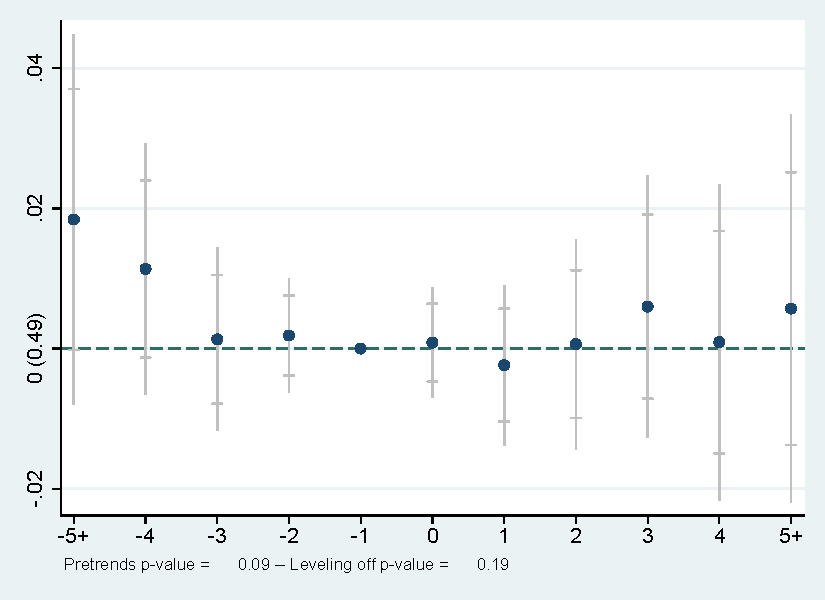
\includegraphics[width=\textwidth]{Objects/xtevent_hosp_fullsample_office.pdf}
            \caption{\small All Physicians \\(Only 1 Hospital)}
        \end{minipage}
        \hspace{0.2cm}
        \begin{minipage}[b]{0.47\linewidth}
            \centering
            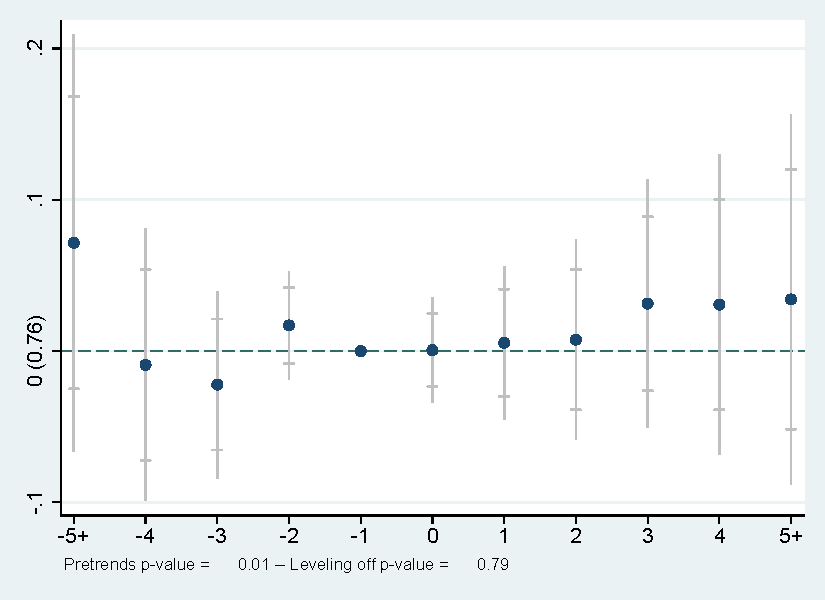
\includegraphics[width=\textwidth]{Objects/xtevent_hosp_oldsample_office.pdf}
            \caption{\small Phys.$>$35yrs Experience\\ (Only 1 Hospital)}
        \end{minipage}
    \end{figure}
\end{frame}


\section{Continuing Work}

\begin{frame}{Plans}
    \begin{itemize}
        \item Analysis on retirement decision of physicians: requires a better understanding of why physicians would drop out of this Medicaid data
    \end{itemize}
\end{frame}



\end{document}
